% Options for packages loaded elsewhere
\PassOptionsToPackage{unicode}{hyperref}
\PassOptionsToPackage{hyphens}{url}
%
\documentclass[
]{article}
\usepackage{amsmath,amssymb}
\usepackage{lmodern}
\usepackage{iftex}
\ifPDFTeX
  \usepackage[T1]{fontenc}
  \usepackage[utf8]{inputenc}
  \usepackage{textcomp} % provide euro and other symbols
\else % if luatex or xetex
  \usepackage{unicode-math}
  \defaultfontfeatures{Scale=MatchLowercase}
  \defaultfontfeatures[\rmfamily]{Ligatures=TeX,Scale=1}
\fi
% Use upquote if available, for straight quotes in verbatim environments
\IfFileExists{upquote.sty}{\usepackage{upquote}}{}
\IfFileExists{microtype.sty}{% use microtype if available
  \usepackage[]{microtype}
  \UseMicrotypeSet[protrusion]{basicmath} % disable protrusion for tt fonts
}{}
\makeatletter
\@ifundefined{KOMAClassName}{% if non-KOMA class
  \IfFileExists{parskip.sty}{%
    \usepackage{parskip}
  }{% else
    \setlength{\parindent}{0pt}
    \setlength{\parskip}{6pt plus 2pt minus 1pt}}
}{% if KOMA class
  \KOMAoptions{parskip=half}}
\makeatother
\usepackage{xcolor}
\usepackage[margin=1in]{geometry}
\usepackage{color}
\usepackage{fancyvrb}
\newcommand{\VerbBar}{|}
\newcommand{\VERB}{\Verb[commandchars=\\\{\}]}
\DefineVerbatimEnvironment{Highlighting}{Verbatim}{commandchars=\\\{\}}
% Add ',fontsize=\small' for more characters per line
\usepackage{framed}
\definecolor{shadecolor}{RGB}{248,248,248}
\newenvironment{Shaded}{\begin{snugshade}}{\end{snugshade}}
\newcommand{\AlertTok}[1]{\textcolor[rgb]{0.94,0.16,0.16}{#1}}
\newcommand{\AnnotationTok}[1]{\textcolor[rgb]{0.56,0.35,0.01}{\textbf{\textit{#1}}}}
\newcommand{\AttributeTok}[1]{\textcolor[rgb]{0.77,0.63,0.00}{#1}}
\newcommand{\BaseNTok}[1]{\textcolor[rgb]{0.00,0.00,0.81}{#1}}
\newcommand{\BuiltInTok}[1]{#1}
\newcommand{\CharTok}[1]{\textcolor[rgb]{0.31,0.60,0.02}{#1}}
\newcommand{\CommentTok}[1]{\textcolor[rgb]{0.56,0.35,0.01}{\textit{#1}}}
\newcommand{\CommentVarTok}[1]{\textcolor[rgb]{0.56,0.35,0.01}{\textbf{\textit{#1}}}}
\newcommand{\ConstantTok}[1]{\textcolor[rgb]{0.00,0.00,0.00}{#1}}
\newcommand{\ControlFlowTok}[1]{\textcolor[rgb]{0.13,0.29,0.53}{\textbf{#1}}}
\newcommand{\DataTypeTok}[1]{\textcolor[rgb]{0.13,0.29,0.53}{#1}}
\newcommand{\DecValTok}[1]{\textcolor[rgb]{0.00,0.00,0.81}{#1}}
\newcommand{\DocumentationTok}[1]{\textcolor[rgb]{0.56,0.35,0.01}{\textbf{\textit{#1}}}}
\newcommand{\ErrorTok}[1]{\textcolor[rgb]{0.64,0.00,0.00}{\textbf{#1}}}
\newcommand{\ExtensionTok}[1]{#1}
\newcommand{\FloatTok}[1]{\textcolor[rgb]{0.00,0.00,0.81}{#1}}
\newcommand{\FunctionTok}[1]{\textcolor[rgb]{0.00,0.00,0.00}{#1}}
\newcommand{\ImportTok}[1]{#1}
\newcommand{\InformationTok}[1]{\textcolor[rgb]{0.56,0.35,0.01}{\textbf{\textit{#1}}}}
\newcommand{\KeywordTok}[1]{\textcolor[rgb]{0.13,0.29,0.53}{\textbf{#1}}}
\newcommand{\NormalTok}[1]{#1}
\newcommand{\OperatorTok}[1]{\textcolor[rgb]{0.81,0.36,0.00}{\textbf{#1}}}
\newcommand{\OtherTok}[1]{\textcolor[rgb]{0.56,0.35,0.01}{#1}}
\newcommand{\PreprocessorTok}[1]{\textcolor[rgb]{0.56,0.35,0.01}{\textit{#1}}}
\newcommand{\RegionMarkerTok}[1]{#1}
\newcommand{\SpecialCharTok}[1]{\textcolor[rgb]{0.00,0.00,0.00}{#1}}
\newcommand{\SpecialStringTok}[1]{\textcolor[rgb]{0.31,0.60,0.02}{#1}}
\newcommand{\StringTok}[1]{\textcolor[rgb]{0.31,0.60,0.02}{#1}}
\newcommand{\VariableTok}[1]{\textcolor[rgb]{0.00,0.00,0.00}{#1}}
\newcommand{\VerbatimStringTok}[1]{\textcolor[rgb]{0.31,0.60,0.02}{#1}}
\newcommand{\WarningTok}[1]{\textcolor[rgb]{0.56,0.35,0.01}{\textbf{\textit{#1}}}}
\usepackage{longtable,booktabs,array}
\usepackage{calc} % for calculating minipage widths
% Correct order of tables after \paragraph or \subparagraph
\usepackage{etoolbox}
\makeatletter
\patchcmd\longtable{\par}{\if@noskipsec\mbox{}\fi\par}{}{}
\makeatother
% Allow footnotes in longtable head/foot
\IfFileExists{footnotehyper.sty}{\usepackage{footnotehyper}}{\usepackage{footnote}}
\makesavenoteenv{longtable}
\usepackage{graphicx}
\makeatletter
\def\maxwidth{\ifdim\Gin@nat@width>\linewidth\linewidth\else\Gin@nat@width\fi}
\def\maxheight{\ifdim\Gin@nat@height>\textheight\textheight\else\Gin@nat@height\fi}
\makeatother
% Scale images if necessary, so that they will not overflow the page
% margins by default, and it is still possible to overwrite the defaults
% using explicit options in \includegraphics[width, height, ...]{}
\setkeys{Gin}{width=\maxwidth,height=\maxheight,keepaspectratio}
% Set default figure placement to htbp
\makeatletter
\def\fps@figure{htbp}
\makeatother
\setlength{\emergencystretch}{3em} % prevent overfull lines
\providecommand{\tightlist}{%
  \setlength{\itemsep}{0pt}\setlength{\parskip}{0pt}}
\setcounter{secnumdepth}{-\maxdimen} % remove section numbering
\ifLuaTeX
  \usepackage{selnolig}  % disable illegal ligatures
\fi
\IfFileExists{bookmark.sty}{\usepackage{bookmark}}{\usepackage{hyperref}}
\IfFileExists{xurl.sty}{\usepackage{xurl}}{} % add URL line breaks if available
\urlstyle{same} % disable monospaced font for URLs
\hypersetup{
  pdftitle={Frequency Analysis of Notes From Portland Harbor Model Workshops},
  pdfauthor={Curtis C. Bohlen},
  hidelinks,
  pdfcreator={LaTeX via pandoc}}

\title{Frequency Analysis of Notes From Portland Harbor Model Workshops}
\author{Curtis C. Bohlen}
\date{2022-12-09}

\begin{document}
\maketitle

{
\setcounter{tocdepth}{2}
\tableofcontents
}
\hypertarget{introduction}{%
\section{Introduction}\label{introduction}}

CBEP recently received a grant from NSF's CIVIC Innovation Challenge to
work on developing hydrodynamic models that address community needs in
Portland Harbor. As part of the project, CBEP hosted three community
workshops in November of 2022.

Facilitators produced both ``live'' notes during the meeting -- visible
to all on a screen at the front of the meeting room -- and detailed
meeting transcripts. CBEP staff then reviewed those notes paragraph by
paragraph, and coded each paragraph in terms of six characteristics:

\begin{itemize}
\item
  Potential users and uses of hydrodynamic models,
\item
  Data or information needs identified by community members,
\item
  Implied extensions of the initial Casco Bay Model required to fully
  address those data needs, and
\item
  Ideas for improving communications of model results (e.g.,
  communications channels and user interface design),
\item
  Specifications for model performance or data criteria such as
  resolution, geographic coverage or ability to conduct simulations.
\item
  Suggestions about monitoring or data collection that could improve
  information availability.
\end{itemize}

If a paragraph or live note included something relevant to one or more
of these categories, we summarized the related idea, and then assigned
each paragraph or comment to categories. In this way we can look at what
ideas were expressed most commonly during the workshops.

Of course, not all paragraphs include information related to each of the
six types of information, so there is not a perfect one-to-one
correspondence between categories.

In this R Notebook, I explore these data in terms of frequency with
which certain ideas came up, and cross-correlations among ideas.

\hypertarget{load-packages}{%
\section{Load Packages}\label{load-packages}}

\begin{Shaded}
\begin{Highlighting}[]
\FunctionTok{library}\NormalTok{(tidyverse)}
\CommentTok{\#\textgreater{} {-}{-} Attaching packages {-}{-}{-}{-}{-}{-}{-}{-}{-}{-}{-}{-}{-}{-}{-}{-}{-}{-}{-}{-}{-}{-}{-}{-}{-}{-}{-}{-}{-}{-}{-}{-}{-}{-}{-}{-}{-}{-}{-} tidyverse 1.3.2 {-}{-}}
\CommentTok{\#\textgreater{} v ggplot2 3.4.0      v purrr   0.3.5 }
\CommentTok{\#\textgreater{} v tibble  3.1.8      v dplyr   1.0.10}
\CommentTok{\#\textgreater{} v tidyr   1.2.1      v stringr 1.5.0 }
\CommentTok{\#\textgreater{} v readr   2.1.3      v forcats 0.5.2 }
\CommentTok{\#\textgreater{} {-}{-} Conflicts {-}{-}{-}{-}{-}{-}{-}{-}{-}{-}{-}{-}{-}{-}{-}{-}{-}{-}{-}{-}{-}{-}{-}{-}{-}{-}{-}{-}{-}{-}{-}{-}{-}{-}{-}{-}{-}{-}{-}{-}{-}{-} tidyverse\_conflicts() {-}{-}}
\CommentTok{\#\textgreater{} x dplyr::filter() masks stats::filter()}
\CommentTok{\#\textgreater{} x dplyr::lag()    masks stats::lag()}
\FunctionTok{library}\NormalTok{(ggmosaic)}
\FunctionTok{library}\NormalTok{(readxl)}
\FunctionTok{library}\NormalTok{(networkD3)}

\FunctionTok{theme\_set}\NormalTok{(}\FunctionTok{theme\_classic}\NormalTok{())}
\end{Highlighting}
\end{Shaded}

\hypertarget{create-figures-folder}{%
\section{Create Figures Folder}\label{create-figures-folder}}

\begin{Shaded}
\begin{Highlighting}[]
\FunctionTok{dir.create}\NormalTok{(}\FunctionTok{file.path}\NormalTok{(}\FunctionTok{getwd}\NormalTok{(), }\StringTok{\textquotesingle{}figures\textquotesingle{}}\NormalTok{), }\AttributeTok{showWarnings =} \ConstantTok{FALSE}\NormalTok{)}
\end{Highlighting}
\end{Shaded}

\hypertarget{load-data}{%
\section{Load Data}\label{load-data}}

\begin{Shaded}
\begin{Highlighting}[]
\NormalTok{the\_data }\OtherTok{\textless{}{-}} \FunctionTok{read\_excel}\NormalTok{(}\StringTok{"Data\_Export\_Query.xlsx"}\NormalTok{ ) }\SpecialCharTok{\%\textgreater{}\%}
  \FunctionTok{mutate}\NormalTok{(}\AttributeTok{ID =} \FunctionTok{as.integer}\NormalTok{(ID)) }\SpecialCharTok{\%\textgreater{}\%}
  \FunctionTok{rename\_with}\NormalTok{(}\ControlFlowTok{function}\NormalTok{(x) }\FunctionTok{sub}\NormalTok{(}\StringTok{" Category\_Category"}\NormalTok{, }\StringTok{\textquotesingle{}\_Category\textquotesingle{}}\NormalTok{, x)) }\SpecialCharTok{\%\textgreater{}\%}
  \FunctionTok{rename\_with}\NormalTok{(}\ControlFlowTok{function}\NormalTok{(x) }\FunctionTok{sub}\NormalTok{(}\StringTok{" "}\NormalTok{, }\StringTok{\textquotesingle{}\_\textquotesingle{}}\NormalTok{, x))}
\FunctionTok{head}\NormalTok{(the\_data)}
\CommentTok{\#\textgreater{} \# A tibble: 6 x 16}
\CommentTok{\#\textgreater{}      ID Category   Day   Comment User\_\textasciitilde{}1 Inter\textasciitilde{}2 Inter\textasciitilde{}3 Data\_\textasciitilde{}4 Data\_\textasciitilde{}5 Exten\textasciitilde{}6}
\CommentTok{\#\textgreater{}   \textless{}int\textgreater{} \textless{}chr\textgreater{}      \textless{}chr\textgreater{} \textless{}chr\textgreater{}   \textless{}chr\textgreater{}   \textless{}chr\textgreater{}   \textless{}chr\textgreater{}   \textless{}chr\textgreater{}     \textless{}dbl\textgreater{} \textless{}chr\textgreater{}  }
\CommentTok{\#\textgreater{} 1     1 Live Comm\textasciitilde{} Day \textasciitilde{} How ca\textasciitilde{} Urban \textasciitilde{} Simple  Exampl\textasciitilde{} \textless{}NA\textgreater{}         NA Draina\textasciitilde{}}
\CommentTok{\#\textgreater{} 2     2 Live Comm\textasciitilde{} Day \textasciitilde{} Use of\textasciitilde{} Harbor\textasciitilde{} \textless{}NA\textgreater{}    \textless{}NA\textgreater{}    Waves         4 \textless{}NA\textgreater{}   }
\CommentTok{\#\textgreater{} 3     2 Live Comm\textasciitilde{} Day \textasciitilde{} Use of\textasciitilde{} Marine\textasciitilde{} \textless{}NA\textgreater{}    \textless{}NA\textgreater{}    Waves         4 \textless{}NA\textgreater{}   }
\CommentTok{\#\textgreater{} 4     2 Live Comm\textasciitilde{} Day \textasciitilde{} Use of\textasciitilde{} Urban \textasciitilde{} \textless{}NA\textgreater{}    \textless{}NA\textgreater{}    Waves         4 \textless{}NA\textgreater{}   }
\CommentTok{\#\textgreater{} 5     3 Live Comm\textasciitilde{} Day \textasciitilde{} MS4 pr\textasciitilde{} Water \textasciitilde{} Inform\textasciitilde{} Shared\textasciitilde{} \textless{}NA\textgreater{}         NA Discha\textasciitilde{}}
\CommentTok{\#\textgreater{} 6     3 Live Comm\textasciitilde{} Day \textasciitilde{} MS4 pr\textasciitilde{} Water \textasciitilde{} Inform\textasciitilde{} Shared\textasciitilde{} \textless{}NA\textgreater{}         NA Draina\textasciitilde{}}
\CommentTok{\#\textgreater{} \# ... with 6 more variables: Extension\_Timing \textless{}dbl\textgreater{}, Monitoring\_Category \textless{}chr\textgreater{},}
\CommentTok{\#\textgreater{} \#   Monitoring\_Data\_Group \textless{}chr\textgreater{}, Data\_Quality\_Category \textless{}chr\textgreater{},}
\CommentTok{\#\textgreater{} \#   Data\_Quality\_Type \textless{}dbl\textgreater{}, Data\_Quality\_Timing \textless{}dbl\textgreater{}, and abbreviated}
\CommentTok{\#\textgreater{} \#   variable names 1: User\_Category, 2: Interface\_Category, 3: Interface\_Group,}
\CommentTok{\#\textgreater{} \#   4: Data\_Group, 5: Data\_Timing, 6: Extension\_Category}
\end{Highlighting}
\end{Shaded}

Our coding was generated in a somewhat sloppy \texttt{Access} database,
and because of the way SQL works, it is easier to replace numerical
values for some groups here, in \texttt{R}, rather than before we
exported the data from \texttt{Access}. I read in the dictionaries here.

\begin{Shaded}
\begin{Highlighting}[]
\NormalTok{timing\_table }\OtherTok{\textless{}{-}} \FunctionTok{read\_excel}\NormalTok{(}\StringTok{"Timing Category.xlsx"}\NormalTok{, }
    \AttributeTok{col\_types =} \FunctionTok{c}\NormalTok{(}\StringTok{"numeric"}\NormalTok{, }\StringTok{"text"}\NormalTok{, }\StringTok{"text"}\NormalTok{))}
\NormalTok{data\_types\_table }\OtherTok{\textless{}{-}} \FunctionTok{read\_excel}\NormalTok{(}\StringTok{"Data Type.xlsx"}\NormalTok{, }
    \AttributeTok{col\_types =} \FunctionTok{c}\NormalTok{(}\StringTok{"numeric"}\NormalTok{, }\StringTok{"text"}\NormalTok{, }\StringTok{"text"}\NormalTok{))}
\end{Highlighting}
\end{Shaded}

\hypertarget{numerical-values-to-strings}{%
\subsection{Numerical Values to
Strings}\label{numerical-values-to-strings}}

And finally I correct the data table to all text entries.

\begin{Shaded}
\begin{Highlighting}[]
\NormalTok{the\_data }\OtherTok{\textless{}{-}}\NormalTok{ the\_data }\SpecialCharTok{\%\textgreater{}\%}
  \FunctionTok{mutate}\NormalTok{(}\AttributeTok{Data\_Timing =}\NormalTok{ timing\_table}\SpecialCharTok{$}\NormalTok{Timing[}\FunctionTok{match}\NormalTok{(Data\_Timing, }
\NormalTok{                                                 timing\_table}\SpecialCharTok{$}\NormalTok{ID)],}
         \AttributeTok{Extension\_Timing =}\NormalTok{ timing\_table}\SpecialCharTok{$}\NormalTok{Timing[}\FunctionTok{match}\NormalTok{(Extension\_Timing,}
\NormalTok{                                                      timing\_table}\SpecialCharTok{$}\NormalTok{ID)],}
         \AttributeTok{Data\_Quality\_Timing =}\NormalTok{ timing\_table}\SpecialCharTok{$}\NormalTok{Timing[}\FunctionTok{match}\NormalTok{(Data\_Quality\_Timing,}
\NormalTok{                                                      timing\_table}\SpecialCharTok{$}\NormalTok{ID)]) }\SpecialCharTok{\%\textgreater{}\%}
  \FunctionTok{mutate}\NormalTok{(}\AttributeTok{Monitoring\_Data\_Group =}\NormalTok{ data\_types\_table}\SpecialCharTok{$}\NormalTok{Group[}\FunctionTok{match}\NormalTok{(Monitoring\_Data\_Group,}
\NormalTok{                                                    data\_types\_table}\SpecialCharTok{$}\NormalTok{ID)],}
         \AttributeTok{Data\_Quality\_Type =}\NormalTok{ data\_types\_table}\SpecialCharTok{$}\NormalTok{Group[}\FunctionTok{match}\NormalTok{(Data\_Quality\_Type,}
\NormalTok{                                                    data\_types\_table}\SpecialCharTok{$}\NormalTok{ID)])}
\end{Highlighting}
\end{Shaded}

\begin{Shaded}
\begin{Highlighting}[]
\NormalTok{the\_data }\SpecialCharTok{\%\textgreater{}\%}
  \FunctionTok{filter}\NormalTok{(}\SpecialCharTok{!} \FunctionTok{is.na}\NormalTok{(Monitoring\_Data\_Group)) }\SpecialCharTok{\%\textgreater{}\%}
  \FunctionTok{select}\NormalTok{(}\FunctionTok{contains}\NormalTok{(}\StringTok{"Monitoring"}\NormalTok{))}
\CommentTok{\#\textgreater{} \# A tibble: 32 x 2}
\CommentTok{\#\textgreater{}    Monitoring\_Category Monitoring\_Data\_Group}
\CommentTok{\#\textgreater{}    \textless{}chr\textgreater{}               \textless{}chr\textgreater{}                }
\CommentTok{\#\textgreater{}  1 Type of Data        Temperature          }
\CommentTok{\#\textgreater{}  2 Type of Data        Temperature          }
\CommentTok{\#\textgreater{}  3 Match to Model      Water Quality        }
\CommentTok{\#\textgreater{}  4 Match to Model      Water Quality        }
\CommentTok{\#\textgreater{}  5 Match to Model      Water Quality        }
\CommentTok{\#\textgreater{}  6 Match to Model      Water Quality        }
\CommentTok{\#\textgreater{}  7 Match to Model      Water Quality        }
\CommentTok{\#\textgreater{}  8 Match to Model      Water Quality        }
\CommentTok{\#\textgreater{}  9 Match to Model      Water Level          }
\CommentTok{\#\textgreater{} 10 Type of Data        Salinity             }
\CommentTok{\#\textgreater{} \# ... with 22 more rows}
\end{Highlighting}
\end{Shaded}

\#A Warning about Uniqueness We have to be careful here, because each
note or comment can be represented in this data table multiple times.
Each paragraph in the meeting transcript might imply several different
users, for example. But if there are multiple users and multiple data
types, the records got duplicated (in part) in the SQL query. So for any
analysis, we need to test for uniqueness of the data. always

We actually have over 375 records, built out of just over 200 unique
comments.

\begin{Shaded}
\begin{Highlighting}[]
\FunctionTok{cat}\NormalTok{(}\StringTok{"All rows in the data:}\SpecialCharTok{\textbackslash{}t\textbackslash{}t}\StringTok{"}\NormalTok{)}
\CommentTok{\#\textgreater{} All rows in the data:        }
\FunctionTok{nrow}\NormalTok{(the\_data)}
\CommentTok{\#\textgreater{} [1] 379}

\FunctionTok{cat}\NormalTok{(}\StringTok{"Unique comments reviewed:}\SpecialCharTok{\textbackslash{}t}\StringTok{"}\NormalTok{)}
\CommentTok{\#\textgreater{} Unique comments reviewed:    }
\NormalTok{the\_data }\SpecialCharTok{\%\textgreater{}\%}
  \FunctionTok{select}\NormalTok{(ID) }\SpecialCharTok{\%\textgreater{}\%}
  \FunctionTok{unique}\NormalTok{() }\SpecialCharTok{\%\textgreater{}\%}
  \FunctionTok{nrow}\NormalTok{()}
\CommentTok{\#\textgreater{} [1] 207}
\end{Highlighting}
\end{Shaded}

\hypertarget{users}{%
\section{Users}\label{users}}

\begin{Shaded}
\begin{Highlighting}[]
\NormalTok{tmp }\OtherTok{\textless{}{-}}\NormalTok{ the\_data }\SpecialCharTok{\%\textgreater{}\%}
  \FunctionTok{select}\NormalTok{(ID, User\_Category) }\SpecialCharTok{\%\textgreater{}\%}
  \FunctionTok{unique}\NormalTok{()}
\NormalTok{tst }\OtherTok{\textless{}{-}} \FunctionTok{xtabs}\NormalTok{(}\SpecialCharTok{\textasciitilde{}}\NormalTok{User\_Category, tmp) }\SpecialCharTok{\%\textgreater{}\%}
  \FunctionTok{sort}\NormalTok{(}\AttributeTok{decreasing =} \ConstantTok{TRUE}\NormalTok{) }\SpecialCharTok{\%\textgreater{}\%}
  \FunctionTok{as\_tibble}\NormalTok{()}


\FunctionTok{cat}\NormalTok{(}\StringTok{"Number of Unique User Records:}\SpecialCharTok{\textbackslash{}t}\StringTok{"}\NormalTok{)}
\CommentTok{\#\textgreater{} Number of Unique User Records:   }
\FunctionTok{sum}\NormalTok{(tst}\SpecialCharTok{$}\NormalTok{n)}
\CommentTok{\#\textgreater{} [1] 191}
\end{Highlighting}
\end{Shaded}

\begin{Shaded}
\begin{Highlighting}[]
\NormalTok{tst }\SpecialCharTok{\%\textgreater{}\%}
  \FunctionTok{mutate}\NormalTok{(}\AttributeTok{User\_Category =} \FunctionTok{fct\_reorder}\NormalTok{(User\_Category, n, }\AttributeTok{.desc =} \ConstantTok{TRUE}\NormalTok{)) }\SpecialCharTok{\%\textgreater{}\%}
  
  \FunctionTok{ggplot}\NormalTok{(}\FunctionTok{aes}\NormalTok{(User\_Category, n)) }\SpecialCharTok{+}
  \FunctionTok{geom\_col}\NormalTok{(}\AttributeTok{fill =} \StringTok{"blue4"}\NormalTok{) }\SpecialCharTok{+}
  \FunctionTok{theme}\NormalTok{(}\AttributeTok{axis.text.x =} \FunctionTok{element\_text}\NormalTok{(}\AttributeTok{angle =} \DecValTok{90}\NormalTok{, }\AttributeTok{size =} \DecValTok{16}\NormalTok{,}
                                   \AttributeTok{hjust =} \DecValTok{1}\NormalTok{, }\AttributeTok{vjust =} \FloatTok{0.25}\NormalTok{)) }\SpecialCharTok{+}
  \FunctionTok{ylab}\NormalTok{(}\StringTok{\textquotesingle{}Count\textquotesingle{}}\NormalTok{) }\SpecialCharTok{+}
  \FunctionTok{xlab}\NormalTok{(}\StringTok{""}\NormalTok{) }\SpecialCharTok{+}
  \FunctionTok{ggtitle}\NormalTok{(}\StringTok{\textquotesingle{}Users\textquotesingle{}}\NormalTok{)}
\end{Highlighting}
\end{Shaded}

\begin{center}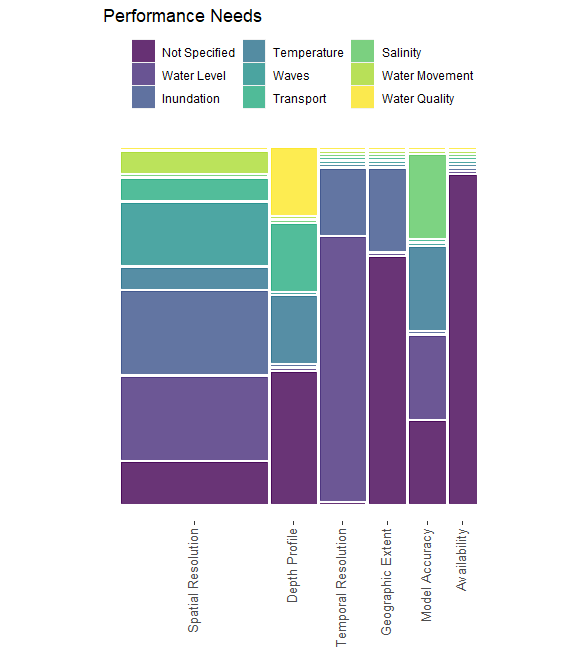
\includegraphics{Initial-Data-Review_files/figure-latex/unnamed-chunk-9-1} \end{center}

\begin{Shaded}
\begin{Highlighting}[]
\FunctionTok{ggsave}\NormalTok{(}\StringTok{\textquotesingle{}figures/users.png\textquotesingle{}}\NormalTok{, }\AttributeTok{type=}\StringTok{\textquotesingle{}cairo\textquotesingle{}}\NormalTok{,}
         \AttributeTok{width =} \DecValTok{6}\NormalTok{, }\AttributeTok{height =} \DecValTok{6}\NormalTok{)}
\end{Highlighting}
\end{Shaded}

\hypertarget{data-types-requested}{%
\section{Data Types Requested}\label{data-types-requested}}

\begin{Shaded}
\begin{Highlighting}[]
\NormalTok{tmp }\OtherTok{\textless{}{-}}\NormalTok{ the\_data }\SpecialCharTok{\%\textgreater{}\%}
  \FunctionTok{select}\NormalTok{(ID, Data\_Group) }\SpecialCharTok{\%\textgreater{}\%}
  \FunctionTok{unique}\NormalTok{()}
\NormalTok{tst }\OtherTok{\textless{}{-}} \FunctionTok{xtabs}\NormalTok{(}\SpecialCharTok{\textasciitilde{}}\NormalTok{Data\_Group, tmp) }\SpecialCharTok{\%\textgreater{}\%}
  \FunctionTok{sort}\NormalTok{(}\AttributeTok{decreasing =} \ConstantTok{TRUE}\NormalTok{) }\SpecialCharTok{\%\textgreater{}\%}
  \FunctionTok{as\_tibble}\NormalTok{()}

\FunctionTok{cat}\NormalTok{(}\StringTok{"Number of Unique Data Records:}\SpecialCharTok{\textbackslash{}t}\StringTok{"}\NormalTok{)}
\CommentTok{\#\textgreater{} Number of Unique Data Records:   }
\FunctionTok{sum}\NormalTok{(tst}\SpecialCharTok{$}\NormalTok{n)}
\CommentTok{\#\textgreater{} [1] 110}
\end{Highlighting}
\end{Shaded}

\begin{Shaded}
\begin{Highlighting}[]
\NormalTok{tmp }\SpecialCharTok{\%\textgreater{}\%}
  \FunctionTok{filter}\NormalTok{(}\SpecialCharTok{!} \FunctionTok{is.na}\NormalTok{(Data\_Group))  }\SpecialCharTok{\%\textgreater{}\%}
  \FunctionTok{mutate}\NormalTok{(}\AttributeTok{Data\_Group =} \FunctionTok{fct\_infreq}\NormalTok{(Data\_Group)) }\SpecialCharTok{\%\textgreater{}\%}
   
  \FunctionTok{ggplot}\NormalTok{(}\FunctionTok{aes}\NormalTok{(Data\_Group)) }\SpecialCharTok{+}
  \FunctionTok{geom\_bar}\NormalTok{(}\AttributeTok{fill =} \StringTok{"blue4"}\NormalTok{) }\SpecialCharTok{+}
  \FunctionTok{theme}\NormalTok{(}\AttributeTok{axis.text.x =} \FunctionTok{element\_text}\NormalTok{(}\AttributeTok{angle =} \DecValTok{90}\NormalTok{, }\AttributeTok{size =} \DecValTok{16}\NormalTok{,}
                                   \AttributeTok{hjust =} \DecValTok{1}\NormalTok{, }\AttributeTok{vjust =} \FloatTok{0.25}\NormalTok{)) }\SpecialCharTok{+}
  \FunctionTok{ylab}\NormalTok{(}\StringTok{\textquotesingle{}Count\textquotesingle{}}\NormalTok{) }\SpecialCharTok{+}
  \FunctionTok{xlab}\NormalTok{(}\StringTok{""}\NormalTok{) }\SpecialCharTok{+}
  \FunctionTok{ggtitle}\NormalTok{(}\StringTok{"Data Types Requested or Implied"}\NormalTok{)}
\end{Highlighting}
\end{Shaded}

\begin{center}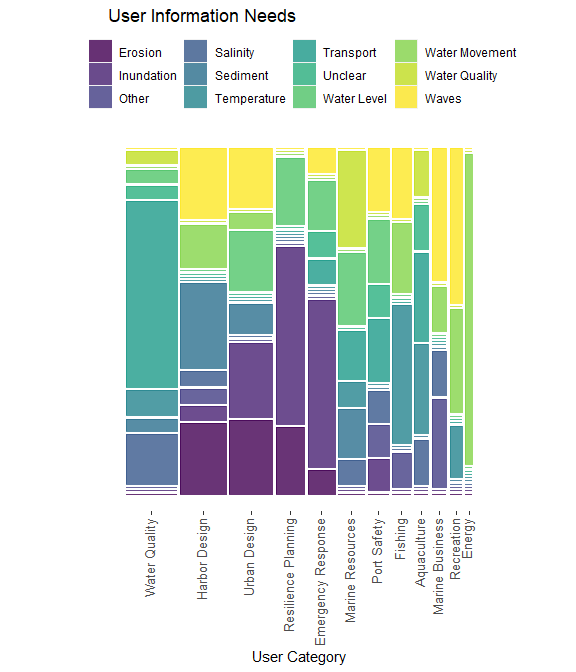
\includegraphics{Initial-Data-Review_files/figure-latex/unnamed-chunk-12-1} \end{center}

\begin{Shaded}
\begin{Highlighting}[]
\FunctionTok{ggsave}\NormalTok{(}\StringTok{\textquotesingle{}figures/data.png\textquotesingle{}}\NormalTok{, }\AttributeTok{type=}\StringTok{\textquotesingle{}cairo\textquotesingle{}}\NormalTok{,}
         \AttributeTok{width =} \DecValTok{6}\NormalTok{, }\AttributeTok{height =} \DecValTok{6}\NormalTok{)}
\end{Highlighting}
\end{Shaded}

\hypertarget{model-extensions}{%
\section{Model Extensions}\label{model-extensions}}

\begin{Shaded}
\begin{Highlighting}[]
\NormalTok{tmp }\OtherTok{\textless{}{-}}\NormalTok{ the\_data }\SpecialCharTok{\%\textgreater{}\%}
  \FunctionTok{select}\NormalTok{(ID, Extension\_Category) }\SpecialCharTok{\%\textgreater{}\%}
  \FunctionTok{unique}\NormalTok{()}
\NormalTok{tst }\OtherTok{\textless{}{-}} \FunctionTok{xtabs}\NormalTok{(}\SpecialCharTok{\textasciitilde{}}\NormalTok{Extension\_Category, tmp) }\SpecialCharTok{\%\textgreater{}\%}
  \FunctionTok{sort}\NormalTok{(}\AttributeTok{decreasing =} \ConstantTok{TRUE}\NormalTok{) }\SpecialCharTok{\%\textgreater{}\%}
  \FunctionTok{as\_tibble}\NormalTok{()}

\FunctionTok{cat}\NormalTok{(}\StringTok{"Number of Unique Extension Records:}\SpecialCharTok{\textbackslash{}t}\StringTok{"}\NormalTok{)}
\CommentTok{\#\textgreater{} Number of Unique Extension Records:  }
\FunctionTok{sum}\NormalTok{(tst}\SpecialCharTok{$}\NormalTok{n)}
\CommentTok{\#\textgreater{} [1] 80}
\end{Highlighting}
\end{Shaded}

\begin{Shaded}
\begin{Highlighting}[]
\NormalTok{tmp }\SpecialCharTok{\%\textgreater{}\%}
  \FunctionTok{filter}\NormalTok{(}\SpecialCharTok{!} \FunctionTok{is.na}\NormalTok{(Extension\_Category))  }\SpecialCharTok{\%\textgreater{}\%}
  \FunctionTok{mutate}\NormalTok{(}\AttributeTok{Extension\_Category =} \FunctionTok{fct\_infreq}\NormalTok{(Extension\_Category)) }\SpecialCharTok{\%\textgreater{}\%}
   
  \FunctionTok{ggplot}\NormalTok{(}\FunctionTok{aes}\NormalTok{(Extension\_Category)) }\SpecialCharTok{+}
  \FunctionTok{geom\_bar}\NormalTok{(}\AttributeTok{fill =} \StringTok{"blue4"}\NormalTok{) }\SpecialCharTok{+}
  \FunctionTok{theme}\NormalTok{(}\AttributeTok{axis.text.x =} \FunctionTok{element\_text}\NormalTok{(}\AttributeTok{angle =} \DecValTok{90}\NormalTok{, }\AttributeTok{size =} \DecValTok{16}\NormalTok{,}
                                   \AttributeTok{hjust =} \DecValTok{1}\NormalTok{, }\AttributeTok{vjust =} \FloatTok{0.25}\NormalTok{)) }\SpecialCharTok{+}
  \FunctionTok{ylab}\NormalTok{(}\StringTok{\textquotesingle{}Count\textquotesingle{}}\NormalTok{) }\SpecialCharTok{+}
  \FunctionTok{xlab}\NormalTok{(}\StringTok{""}\NormalTok{) }\SpecialCharTok{+}
  \FunctionTok{ggtitle}\NormalTok{(}\StringTok{"Additional Models or Model Extensions Implied"}\NormalTok{)}
\end{Highlighting}
\end{Shaded}

\begin{center}\includegraphics{Initial-Data-Review_files/figure-latex/unnamed-chunk-15-1} \end{center}

\begin{Shaded}
\begin{Highlighting}[]
\FunctionTok{ggsave}\NormalTok{(}\StringTok{\textquotesingle{}figures/models.png\textquotesingle{}}\NormalTok{, }\AttributeTok{type=}\StringTok{\textquotesingle{}cairo\textquotesingle{}}\NormalTok{,}
         \AttributeTok{width =} \DecValTok{6}\NormalTok{, }\AttributeTok{height =} \DecValTok{6}\NormalTok{)}
\end{Highlighting}
\end{Shaded}

\hypertarget{what-are-the-comments-associated-with-the-other-category}{%
\subsection{What are the comments associated with the ``Other''
Category?}\label{what-are-the-comments-associated-with-the-other-category}}

\begin{Shaded}
\begin{Highlighting}[]
\NormalTok{the\_data }\SpecialCharTok{\%\textgreater{}\%}
  \FunctionTok{filter}\NormalTok{(Extension\_Category }\SpecialCharTok{==} \StringTok{"Other"}\NormalTok{) }\SpecialCharTok{\%\textgreater{}\%}
  \FunctionTok{select}\NormalTok{(ID, Comment) }\SpecialCharTok{\%\textgreater{}\%}
  \FunctionTok{unique}\NormalTok{()}\SpecialCharTok{\%\textgreater{}\%}
  \FunctionTok{pull}\NormalTok{(Comment)}
\CommentTok{\#\textgreater{} [1] "Saltwater intrusion into isolated aquifers – impacts on local (peninsular and island) aquifers"                                                                                                                                                                 }
\CommentTok{\#\textgreater{} [2] "Kelp, shellfish, other aquatic resources – are rapidly expanding in Casco Bay – so re impacted by nutrient / pollutant loading.  There is a  question of siting aquaculture and managing those facilities.  Can the model inform that issue?  It is important t"}
\CommentTok{\#\textgreater{} [3] "* Saltwater intrusion into isolated aquifers – impacts on local (peninsular and island) aquifers"                                                                                                                                                               }
\CommentTok{\#\textgreater{} [4] "* Modeling of saltwater intrusion can benefit from better understanding of nearshore coastal water"}
\end{Highlighting}
\end{Shaded}

So the model extensions I classified as ``Other'' include: * Developing
decision support tools for aquaculture siting and permitting; and

\begin{itemize}
\tightlist
\item
  Modelling impact of rising seas on groundwater.
\end{itemize}

\hypertarget{user-interface-ideas}{%
\section{User Interface Ideas}\label{user-interface-ideas}}

\begin{Shaded}
\begin{Highlighting}[]
\NormalTok{tmp }\OtherTok{\textless{}{-}}\NormalTok{ the\_data }\SpecialCharTok{\%\textgreater{}\%}
  \FunctionTok{select}\NormalTok{(ID, Interface\_Category) }\SpecialCharTok{\%\textgreater{}\%}
  \FunctionTok{unique}\NormalTok{()}
\NormalTok{tst }\OtherTok{\textless{}{-}} \FunctionTok{xtabs}\NormalTok{(}\SpecialCharTok{\textasciitilde{}}\NormalTok{Interface\_Category, tmp) }\SpecialCharTok{\%\textgreater{}\%}
  \FunctionTok{sort}\NormalTok{(}\AttributeTok{decreasing =} \ConstantTok{TRUE}\NormalTok{) }\SpecialCharTok{\%\textgreater{}\%}
  \FunctionTok{as\_tibble}\NormalTok{()}

\FunctionTok{cat}\NormalTok{(}\StringTok{"Number of Unique Interface Records:}\SpecialCharTok{\textbackslash{}t}\StringTok{"}\NormalTok{)}
\CommentTok{\#\textgreater{} Number of Unique Interface Records:  }
\FunctionTok{sum}\NormalTok{(tst}\SpecialCharTok{$}\NormalTok{n)}
\CommentTok{\#\textgreater{} [1] 75}
\end{Highlighting}
\end{Shaded}

\begin{Shaded}
\begin{Highlighting}[]
\NormalTok{tmp }\SpecialCharTok{\%\textgreater{}\%}
  \FunctionTok{filter}\NormalTok{(}\SpecialCharTok{!} \FunctionTok{is.na}\NormalTok{(Interface\_Category))  }\SpecialCharTok{\%\textgreater{}\%}
  \FunctionTok{mutate}\NormalTok{(}\AttributeTok{Interface\_Category =} \FunctionTok{fct\_infreq}\NormalTok{(Interface\_Category)) }\SpecialCharTok{\%\textgreater{}\%}
   
  \FunctionTok{ggplot}\NormalTok{(}\FunctionTok{aes}\NormalTok{(Interface\_Category)) }\SpecialCharTok{+}
  \FunctionTok{geom\_bar}\NormalTok{(}\AttributeTok{fill =} \StringTok{"blue4"}\NormalTok{) }\SpecialCharTok{+}

  \FunctionTok{theme}\NormalTok{(}\AttributeTok{axis.text.x =} \FunctionTok{element\_text}\NormalTok{(}\AttributeTok{angle =} \DecValTok{90}\NormalTok{, }\AttributeTok{size =} \DecValTok{16}\NormalTok{,}
                                   \AttributeTok{hjust =} \DecValTok{1}\NormalTok{, }\AttributeTok{vjust =} \FloatTok{0.25}\NormalTok{)) }\SpecialCharTok{+}
  \FunctionTok{ylab}\NormalTok{(}\StringTok{\textquotesingle{}Count\textquotesingle{}}\NormalTok{) }\SpecialCharTok{+}
  \FunctionTok{xlab}\NormalTok{(}\StringTok{""}\NormalTok{) }\SpecialCharTok{+}
  \FunctionTok{ggtitle}\NormalTok{(}\StringTok{"User Interface or Presentation Ideas"}\NormalTok{)}
\end{Highlighting}
\end{Shaded}

\begin{center}\includegraphics{Initial-Data-Review_files/figure-latex/unnamed-chunk-19-1} \end{center}

\begin{Shaded}
\begin{Highlighting}[]
\FunctionTok{ggsave}\NormalTok{(}\StringTok{\textquotesingle{}figures/interfaces.png\textquotesingle{}}\NormalTok{, }\AttributeTok{type=}\StringTok{\textquotesingle{}cairo\textquotesingle{}}\NormalTok{,}
         \AttributeTok{width =} \DecValTok{6}\NormalTok{, }\AttributeTok{height =} \DecValTok{6}\NormalTok{)}
\end{Highlighting}
\end{Shaded}

\hypertarget{what-are-the-comments-associated-with-the-other-category-1}{%
\subsection{What are the comments associated with the ``Other''
Category?}\label{what-are-the-comments-associated-with-the-other-category-1}}

\begin{Shaded}
\begin{Highlighting}[]
\NormalTok{the\_data }\SpecialCharTok{\%\textgreater{}\%}
  \FunctionTok{filter}\NormalTok{(Interface\_Category }\SpecialCharTok{==} \StringTok{"Other"}\NormalTok{) }\SpecialCharTok{\%\textgreater{}\%}
  \FunctionTok{select}\NormalTok{(Comment) }\SpecialCharTok{\%\textgreater{}\%}
  \FunctionTok{unique}\NormalTok{() }\SpecialCharTok{\%\textgreater{}\%}
  \FunctionTok{pull}\NormalTok{()}
\CommentTok{\#\textgreater{}  [1] "Identifying vulnerable infrastructure – so can seek funding to mitigate. Erosion, etc. problems that can impact infrastructure."                                                                                                                                }
\CommentTok{\#\textgreater{}  [2] "What happens to Rt. 1 across marsh area? – need high resolution."                                                                                                                                                                                               }
\CommentTok{\#\textgreater{}  [3] "What are decisions people need to make?  Understand those, so can tailor info shared better."                                                                                                                                                                   }
\CommentTok{\#\textgreater{}  [4] "Need user guides! Make models / tools accessible! (visuals with description). Print option.  Video instructions?"                                                                                                                                               }
\CommentTok{\#\textgreater{}  [5] "Sedimentation rates – inform decisions about dredging.  Location specific. Also sources of sedimentation – from development, scouring of water sources, weather events. (sediment transport info should be available from models, but not estimates of total am"}
\CommentTok{\#\textgreater{}  [6] "Model as a design tool – inform development design.   E.g., test out ideas for built environment. How can models / tools inform design for resiliency?  Developers, property owners, architects, planners, etc. – what happens to wave energy, height, angle of"}
\CommentTok{\#\textgreater{}  [7] "Can models inform re{-}writing of flood ordinances?  Remapping flood zones? How to evacuate, where to build critical infrastructure."                                                                                                                             }
\CommentTok{\#\textgreater{}  [8] "How to highlight place based connections (education) – visualizations, data that can use for education."                                                                                                                                                        }
\CommentTok{\#\textgreater{}  [9] "Where does effluent from wastewater facilities go (old info based on dye studies) – can model provide better info?"                                                                                                                                             }
\CommentTok{\#\textgreater{} [10] "Can use models to predict success of resilience actions? (near shore)  Where to focus efforts?"                                                                                                                                                                 }
\CommentTok{\#\textgreater{} [11] "From chat:  The one meter depth resolution just discussed with regard to wastewater effluent modeling would be fine. I am the DEP modeler."                                                                                                                     }
\CommentTok{\#\textgreater{} [12] "How can the work of modeling contribute to city planning – e.g., stormwater, land{-}based precipitation, sediment flow, pollution, input into the harbor and infrastructure development"}
\end{Highlighting}
\end{Shaded}

\hypertarget{data-quality-or-model-performance-goals}{%
\section{Data Quality or Model Performance
Goals}\label{data-quality-or-model-performance-goals}}

\begin{Shaded}
\begin{Highlighting}[]
\NormalTok{tmp }\OtherTok{\textless{}{-}}\NormalTok{ the\_data }\SpecialCharTok{\%\textgreater{}\%}
  \FunctionTok{select}\NormalTok{(ID, Data\_Quality\_Category, Data\_Quality\_Type, Data\_Quality\_Timing) }\SpecialCharTok{\%\textgreater{}\%}
  \FunctionTok{unique}\NormalTok{() }\SpecialCharTok{\%\textgreater{}\%}
  \FunctionTok{filter}\NormalTok{(}\FunctionTok{if\_any}\NormalTok{(}\FunctionTok{starts\_with}\NormalTok{(}\StringTok{\textquotesingle{}Data\_\textquotesingle{}}\NormalTok{), }\SpecialCharTok{\textasciitilde{}!}\FunctionTok{is.na}\NormalTok{(.)))}

\FunctionTok{xtabs}\NormalTok{(}\SpecialCharTok{\textasciitilde{}}\NormalTok{  Data\_Quality\_Type }\SpecialCharTok{+}\NormalTok{ Data\_Quality\_Category, }\AttributeTok{data =}\NormalTok{ tmp) }\SpecialCharTok{\%\textgreater{}\%}
  \FunctionTok{as\_tibble}\NormalTok{() }\SpecialCharTok{\%\textgreater{}\%}
  \FunctionTok{pivot\_wider}\NormalTok{(}\AttributeTok{names\_from =}\NormalTok{ Data\_Quality\_Type, }\AttributeTok{values\_from =}\NormalTok{ n) }\SpecialCharTok{\%\textgreater{}\%}
  \FunctionTok{mutate}\NormalTok{(}\AttributeTok{row\_tot =} \FunctionTok{rowSums}\NormalTok{(}\FunctionTok{select}\NormalTok{(., }\StringTok{\textasciigrave{}}\AttributeTok{Inundation}\StringTok{\textasciigrave{}}\SpecialCharTok{:}\StringTok{\textasciigrave{}}\AttributeTok{Waves}\StringTok{\textasciigrave{}}\NormalTok{))) }\SpecialCharTok{\%\textgreater{}\%}
  \FunctionTok{arrange}\NormalTok{(}\FunctionTok{desc}\NormalTok{(row\_tot)) }\SpecialCharTok{\%\textgreater{}\%}
\NormalTok{  knitr}\SpecialCharTok{::}\FunctionTok{kable}\NormalTok{()}
\end{Highlighting}
\end{Shaded}

\begin{longtable}[]{@{}
  >{\raggedright\arraybackslash}p{(\columnwidth - 20\tabcolsep) * \real{0.1654}}
  >{\raggedleft\arraybackslash}p{(\columnwidth - 20\tabcolsep) * \real{0.0827}}
  >{\raggedleft\arraybackslash}p{(\columnwidth - 20\tabcolsep) * \real{0.1053}}
  >{\raggedleft\arraybackslash}p{(\columnwidth - 20\tabcolsep) * \real{0.0677}}
  >{\raggedleft\arraybackslash}p{(\columnwidth - 20\tabcolsep) * \real{0.0902}}
  >{\raggedleft\arraybackslash}p{(\columnwidth - 20\tabcolsep) * \real{0.0752}}
  >{\raggedleft\arraybackslash}p{(\columnwidth - 20\tabcolsep) * \real{0.0902}}
  >{\raggedleft\arraybackslash}p{(\columnwidth - 20\tabcolsep) * \real{0.1128}}
  >{\raggedleft\arraybackslash}p{(\columnwidth - 20\tabcolsep) * \real{0.1053}}
  >{\raggedleft\arraybackslash}p{(\columnwidth - 20\tabcolsep) * \real{0.0451}}
  >{\raggedleft\arraybackslash}p{(\columnwidth - 20\tabcolsep) * \real{0.0602}}@{}}
\toprule()
\begin{minipage}[b]{\linewidth}\raggedright
Data\_Quality\_Category
\end{minipage} & \begin{minipage}[b]{\linewidth}\raggedleft
Inundation
\end{minipage} & \begin{minipage}[b]{\linewidth}\raggedleft
Not Specified
\end{minipage} & \begin{minipage}[b]{\linewidth}\raggedleft
Salinity
\end{minipage} & \begin{minipage}[b]{\linewidth}\raggedleft
Temperature
\end{minipage} & \begin{minipage}[b]{\linewidth}\raggedleft
Transport
\end{minipage} & \begin{minipage}[b]{\linewidth}\raggedleft
Water Level
\end{minipage} & \begin{minipage}[b]{\linewidth}\raggedleft
Water Movement
\end{minipage} & \begin{minipage}[b]{\linewidth}\raggedleft
Water Quality
\end{minipage} & \begin{minipage}[b]{\linewidth}\raggedleft
Waves
\end{minipage} & \begin{minipage}[b]{\linewidth}\raggedleft
row\_tot
\end{minipage} \\
\midrule()
\endhead
Spatial Resolution & 4 & 2 & 0 & 1 & 1 & 4 & 1 & 0 & 3 & 16 \\
Timing & 0 & 6 & 0 & 0 & 0 & 1 & 0 & 0 & 0 & 7 \\
Depth Profile & 0 & 2 & 0 & 1 & 1 & 0 & 0 & 1 & 0 & 5 \\
Temporal Resolution & 1 & 0 & 0 & 0 & 0 & 4 & 0 & 0 & 0 & 5 \\
Geographic Extent & 1 & 3 & 0 & 0 & 0 & 0 & 0 & 0 & 0 & 4 \\
Model Accuracy & 0 & 1 & 1 & 1 & 0 & 1 & 0 & 0 & 0 & 4 \\
Availability & 0 & 3 & 0 & 0 & 0 & 0 & 0 & 0 & 0 & 3 \\
\bottomrule()
\end{longtable}

\begin{Shaded}
\begin{Highlighting}[]
\NormalTok{tmp }\SpecialCharTok{\%\textgreater{}\%}
  \FunctionTok{filter}\NormalTok{(}\SpecialCharTok{!} \FunctionTok{is.na}\NormalTok{(Data\_Quality\_Category))  }\SpecialCharTok{\%\textgreater{}\%}
  \FunctionTok{mutate}\NormalTok{(}\AttributeTok{Data\_Quality\_Category =} \FunctionTok{fct\_infreq}\NormalTok{(Data\_Quality\_Category)) }\SpecialCharTok{\%\textgreater{}\%}
  \FunctionTok{mutate}\NormalTok{(}\AttributeTok{Data\_Quality\_Type =} \FunctionTok{fct\_infreq}\NormalTok{(Data\_Quality\_Type)) }\SpecialCharTok{\%\textgreater{}\%}
   
  \FunctionTok{ggplot}\NormalTok{(}\FunctionTok{aes}\NormalTok{(Data\_Quality\_Category)) }\SpecialCharTok{+}
  \FunctionTok{geom\_bar}\NormalTok{(}\FunctionTok{aes}\NormalTok{(}\AttributeTok{fill =}\NormalTok{ Data\_Quality\_Type)) }\SpecialCharTok{+}
  \FunctionTok{theme}\NormalTok{(}\AttributeTok{axis.text.x =} \FunctionTok{element\_text}\NormalTok{(}\AttributeTok{angle =} \DecValTok{90}\NormalTok{, }\AttributeTok{size =} \DecValTok{16}\NormalTok{,}
                                   \AttributeTok{hjust =} \DecValTok{1}\NormalTok{, }\AttributeTok{vjust =} \FloatTok{0.25}\NormalTok{)) }\SpecialCharTok{+}
  \FunctionTok{scale\_fill\_viridis\_d}\NormalTok{(}\AttributeTok{name =} \StringTok{\textquotesingle{}Data Type\textquotesingle{}}\NormalTok{) }\SpecialCharTok{+}
  \FunctionTok{ylab}\NormalTok{(}\StringTok{\textquotesingle{}Count\textquotesingle{}}\NormalTok{) }\SpecialCharTok{+}
  \FunctionTok{xlab}\NormalTok{(}\StringTok{""}\NormalTok{) }\SpecialCharTok{+}
  \FunctionTok{ggtitle}\NormalTok{(}\StringTok{"Performance Suggestions"}\NormalTok{)}
\end{Highlighting}
\end{Shaded}

\begin{center}\includegraphics{Initial-Data-Review_files/figure-latex/unnamed-chunk-23-1} \end{center}

\begin{Shaded}
\begin{Highlighting}[]
\FunctionTok{ggsave}\NormalTok{(}\StringTok{\textquotesingle{}figures/performance.png\textquotesingle{}}\NormalTok{, }\AttributeTok{type=}\StringTok{\textquotesingle{}cairo\textquotesingle{}}\NormalTok{,}
         \AttributeTok{width =} \DecValTok{6}\NormalTok{, }\AttributeTok{height =} \DecValTok{6}\NormalTok{)}
\end{Highlighting}
\end{Shaded}

\begin{Shaded}
\begin{Highlighting}[]
\NormalTok{tmp }\SpecialCharTok{\%\textgreater{}\%}
  \FunctionTok{filter}\NormalTok{(}\SpecialCharTok{!} \FunctionTok{is.na}\NormalTok{(Data\_Quality\_Category))  }\SpecialCharTok{\%\textgreater{}\%}
  \FunctionTok{mutate}\NormalTok{(}\AttributeTok{Data\_Quality\_Category =} \FunctionTok{fct\_infreq}\NormalTok{(Data\_Quality\_Category)) }\SpecialCharTok{\%\textgreater{}\%}
  \FunctionTok{mutate}\NormalTok{(}\AttributeTok{Data\_Quality\_Timing =} \FunctionTok{fct\_infreq}\NormalTok{(Data\_Quality\_Timing)) }\SpecialCharTok{\%\textgreater{}\%}
   
  \FunctionTok{ggplot}\NormalTok{(}\FunctionTok{aes}\NormalTok{(Data\_Quality\_Category)) }\SpecialCharTok{+}
  \FunctionTok{geom\_bar}\NormalTok{(}\FunctionTok{aes}\NormalTok{(}\AttributeTok{fill =}\NormalTok{ Data\_Quality\_Timing)) }\SpecialCharTok{+}
  \FunctionTok{theme}\NormalTok{(}\AttributeTok{axis.text.x =} \FunctionTok{element\_text}\NormalTok{(}\AttributeTok{angle =} \DecValTok{90}\NormalTok{, }\AttributeTok{size =} \DecValTok{16}\NormalTok{,}
                                   \AttributeTok{hjust =} \DecValTok{1}\NormalTok{, }\AttributeTok{vjust =} \FloatTok{0.25}\NormalTok{)) }\SpecialCharTok{+}
  \FunctionTok{scale\_fill\_viridis\_d}\NormalTok{(}\AttributeTok{name =} \StringTok{\textquotesingle{}Data Timing\textquotesingle{}}\NormalTok{) }\SpecialCharTok{+}
  \FunctionTok{ylab}\NormalTok{(}\StringTok{\textquotesingle{}Count\textquotesingle{}}\NormalTok{) }\SpecialCharTok{+}
  \FunctionTok{xlab}\NormalTok{(}\StringTok{""}\NormalTok{) }\SpecialCharTok{+}
  \FunctionTok{ggtitle}\NormalTok{(}\StringTok{"Performance Suggestions"}\NormalTok{)}
\end{Highlighting}
\end{Shaded}

\begin{center}\includegraphics{Initial-Data-Review_files/figure-latex/unnamed-chunk-25-1} \end{center}

\begin{Shaded}
\begin{Highlighting}[]
\FunctionTok{ggsave}\NormalTok{(}\StringTok{\textquotesingle{}figures/performance\_Version 2.png\textquotesingle{}}\NormalTok{, }\AttributeTok{type=}\StringTok{\textquotesingle{}cairo\textquotesingle{}}\NormalTok{,}
         \AttributeTok{width =} \DecValTok{6}\NormalTok{, }\AttributeTok{height =} \DecValTok{6}\NormalTok{)}
\end{Highlighting}
\end{Shaded}

\hypertarget{testing-mosaic-plots}{%
\subsection{Testing Mosaic Plots}\label{testing-mosaic-plots}}

The `ggmosaic' package allows modaic plots, but it's a but buggy and
hard to use.

\begin{Shaded}
\begin{Highlighting}[]
\NormalTok{tmp }\OtherTok{\textless{}{-}}\NormalTok{ tmp }\SpecialCharTok{\%\textgreater{}\%}
  \FunctionTok{filter}\NormalTok{(}\SpecialCharTok{!} \FunctionTok{is.na}\NormalTok{(Data\_Quality\_Category))  }\SpecialCharTok{\%\textgreater{}\%}
  \FunctionTok{mutate}\NormalTok{(}\AttributeTok{Data\_Quality\_Category =} \FunctionTok{fct\_infreq}\NormalTok{(Data\_Quality\_Category),}
         \AttributeTok{Data\_Quality\_Type =} \FunctionTok{fct\_infreq}\NormalTok{(Data\_Quality\_Type),}
         \AttributeTok{Data\_Quality\_Timing =} \FunctionTok{fct\_infreq}\NormalTok{(Data\_Quality\_Timing))}
\end{Highlighting}
\end{Shaded}

\begin{Shaded}
\begin{Highlighting}[]
\FunctionTok{ggplot}\NormalTok{(tmp) }\SpecialCharTok{+}
  \FunctionTok{geom\_mosaic}\NormalTok{(}\FunctionTok{aes}\NormalTok{(}\AttributeTok{x =} \FunctionTok{product}\NormalTok{(Data\_Quality\_Category), }
                  \AttributeTok{fill =}\NormalTok{ Data\_Quality\_Type)) }\SpecialCharTok{+}
  \FunctionTok{scale\_fill\_viridis\_d}\NormalTok{(}\AttributeTok{name =} \StringTok{\textquotesingle{}Timing\textquotesingle{}}\NormalTok{) }\SpecialCharTok{+}
    \FunctionTok{theme}\NormalTok{(}\AttributeTok{axis.text.x =} \FunctionTok{element\_text}\NormalTok{(}\AttributeTok{angle =} \DecValTok{90}\NormalTok{))}
\CommentTok{\#\textgreater{} Warning: \textasciigrave{}unite\_()\textasciigrave{} was deprecated in tidyr 1.2.0.}
\CommentTok{\#\textgreater{} i Please use \textasciigrave{}unite()\textasciigrave{} instead.}
\CommentTok{\#\textgreater{} i The deprecated feature was likely used in the ggmosaic package.}
\CommentTok{\#\textgreater{}   Please report the issue at \textless{}]8;;https://github.com/haleyjeppson/ggmosaichttps://github.com/haleyjeppson/ggmosaic]8;;\textgreater{}.}
\end{Highlighting}
\end{Shaded}

\begin{center}\includegraphics{Initial-Data-Review_files/figure-latex/unnamed-chunk-28-1} \end{center}

\begin{Shaded}
\begin{Highlighting}[]
  \FunctionTok{ggtitle}\NormalTok{(}\StringTok{"Performance Suggestions"}\NormalTok{)}
\CommentTok{\#\textgreater{} $title}
\CommentTok{\#\textgreater{} [1] "Performance Suggestions"}
\CommentTok{\#\textgreater{} }
\CommentTok{\#\textgreater{} attr(,"class")}
\CommentTok{\#\textgreater{} [1] "labels"}
\end{Highlighting}
\end{Shaded}

\begin{Shaded}
\begin{Highlighting}[]
\NormalTok{  tst }\OtherTok{\textless{}{-}} \FunctionTok{ggplot}\NormalTok{(tmp) }\SpecialCharTok{+}
  \FunctionTok{geom\_mosaic}\NormalTok{(}\FunctionTok{aes}\NormalTok{(}\AttributeTok{x =} \FunctionTok{product}\NormalTok{(Data\_Quality\_Category), }\AttributeTok{fill =}\NormalTok{ Data\_Quality\_Type, }
                 \AttributeTok{conds =} \FunctionTok{product}\NormalTok{(Data\_Quality\_Timing))) }\SpecialCharTok{+}
  \FunctionTok{scale\_fill\_viridis\_d}\NormalTok{(}\AttributeTok{name =} \StringTok{\textquotesingle{}Timing\textquotesingle{}}\NormalTok{) }\SpecialCharTok{+}
    \FunctionTok{theme}\NormalTok{(}\AttributeTok{axis.text.x =} \FunctionTok{element\_text}\NormalTok{(}\AttributeTok{angle =} \DecValTok{90}\NormalTok{))}
  \FunctionTok{ggtitle}\NormalTok{(}\StringTok{"Performance Suggestions"}\NormalTok{)}
\CommentTok{\#\textgreater{} $title}
\CommentTok{\#\textgreater{} [1] "Performance Suggestions"}
\CommentTok{\#\textgreater{} }
\CommentTok{\#\textgreater{} attr(,"class")}
\CommentTok{\#\textgreater{} [1] "labels"}
  \FunctionTok{print}\NormalTok{(tst)}
\end{Highlighting}
\end{Shaded}

\begin{center}\includegraphics{Initial-Data-Review_files/figure-latex/unnamed-chunk-29-1} \end{center}

\begin{Shaded}
\begin{Highlighting}[]
\NormalTok{  tst }\OtherTok{\textless{}{-}} \FunctionTok{ggplot}\NormalTok{(tmp) }\SpecialCharTok{+}
  \FunctionTok{geom\_mosaic}\NormalTok{(}\FunctionTok{aes}\NormalTok{(}\AttributeTok{x =} \FunctionTok{product}\NormalTok{(Data\_Quality\_Category), }\AttributeTok{fill =}\NormalTok{ Data\_Quality\_Type)) }\SpecialCharTok{+}
  \FunctionTok{scale\_fill\_viridis\_d}\NormalTok{(}\AttributeTok{name =} \StringTok{\textquotesingle{}Data Type\textquotesingle{}}\NormalTok{) }\SpecialCharTok{+}
  \FunctionTok{theme}\NormalTok{(}\AttributeTok{axis.text.x =} \FunctionTok{element\_text}\NormalTok{(}\AttributeTok{angle =} \DecValTok{30}\NormalTok{, }\AttributeTok{hjust =} \DecValTok{1}\NormalTok{),}
        \AttributeTok{axis.text.y =} \FunctionTok{element\_text}\NormalTok{(}\AttributeTok{angle =} \DecValTok{30}\NormalTok{, }\AttributeTok{hjust =} \DecValTok{1}\NormalTok{)) }\SpecialCharTok{+}
  \FunctionTok{facet\_wrap}\NormalTok{(}\SpecialCharTok{\textasciitilde{}}\NormalTok{Data\_Quality\_Timing,}\AttributeTok{scales =} \StringTok{\textquotesingle{}free\textquotesingle{}}\NormalTok{)}
  \FunctionTok{ggtitle}\NormalTok{(}\StringTok{"Performance Suggestions"}\NormalTok{)}
\CommentTok{\#\textgreater{} $title}
\CommentTok{\#\textgreater{} [1] "Performance Suggestions"}
\CommentTok{\#\textgreater{} }
\CommentTok{\#\textgreater{} attr(,"class")}
\CommentTok{\#\textgreater{} [1] "labels"}
  \FunctionTok{print}\NormalTok{(tst)}
\end{Highlighting}
\end{Shaded}

\begin{center}\includegraphics{Initial-Data-Review_files/figure-latex/unnamed-chunk-30-1} \end{center}

\hypertarget{monitoring-suggestions}{%
\section{Monitoring Suggestions}\label{monitoring-suggestions}}

\begin{Shaded}
\begin{Highlighting}[]
\NormalTok{tmp }\OtherTok{\textless{}{-}}\NormalTok{ the\_data }\SpecialCharTok{\%\textgreater{}\%}
  \FunctionTok{select}\NormalTok{(ID, Monitoring\_Data\_Group) }\SpecialCharTok{\%\textgreater{}\%}
  \FunctionTok{unique}\NormalTok{()}
\NormalTok{tst }\OtherTok{\textless{}{-}} \FunctionTok{xtabs}\NormalTok{(}\SpecialCharTok{\textasciitilde{}}\NormalTok{Monitoring\_Data\_Group, tmp) }\SpecialCharTok{\%\textgreater{}\%}
  \FunctionTok{sort}\NormalTok{(}\AttributeTok{decreasing =} \ConstantTok{TRUE}\NormalTok{) }\SpecialCharTok{\%\textgreater{}\%}
  \FunctionTok{as\_tibble}\NormalTok{()}

\FunctionTok{cat}\NormalTok{(}\StringTok{"Number of Unique Extension Records:}\SpecialCharTok{\textbackslash{}t}\StringTok{"}\NormalTok{)}
\CommentTok{\#\textgreater{} Number of Unique Extension Records:  }
\FunctionTok{sum}\NormalTok{(tst}\SpecialCharTok{$}\NormalTok{n)}
\CommentTok{\#\textgreater{} [1] 27}
\end{Highlighting}
\end{Shaded}

\begin{Shaded}
\begin{Highlighting}[]
\NormalTok{tmp }\SpecialCharTok{\%\textgreater{}\%}
  \FunctionTok{filter}\NormalTok{(}\SpecialCharTok{!} \FunctionTok{is.na}\NormalTok{(Monitoring\_Data\_Group))  }\SpecialCharTok{\%\textgreater{}\%}
  \FunctionTok{mutate}\NormalTok{(}\AttributeTok{Monitoring\_Data\_Group =} \FunctionTok{fct\_infreq}\NormalTok{(Monitoring\_Data\_Group)) }\SpecialCharTok{\%\textgreater{}\%}
   
  \FunctionTok{ggplot}\NormalTok{(}\FunctionTok{aes}\NormalTok{(Monitoring\_Data\_Group)) }\SpecialCharTok{+}
  \FunctionTok{geom\_bar}\NormalTok{(}\AttributeTok{fill =} \StringTok{"blue4"}\NormalTok{) }\SpecialCharTok{+}
  \FunctionTok{theme}\NormalTok{(}\AttributeTok{axis.text.x =} \FunctionTok{element\_text}\NormalTok{(}\AttributeTok{angle =} \DecValTok{90}\NormalTok{, }\AttributeTok{size =} \DecValTok{16}\NormalTok{,}
                                   \AttributeTok{hjust =} \DecValTok{1}\NormalTok{, }\AttributeTok{vjust =} \FloatTok{0.25}\NormalTok{)) }\SpecialCharTok{+}
  \FunctionTok{ylab}\NormalTok{(}\StringTok{\textquotesingle{}Count\textquotesingle{}}\NormalTok{) }\SpecialCharTok{+}
  \FunctionTok{xlab}\NormalTok{(}\StringTok{""}\NormalTok{) }\SpecialCharTok{+}
  \FunctionTok{ggtitle}\NormalTok{(}\StringTok{"Additional Models or Model Extensions Implied"}\NormalTok{)}
\end{Highlighting}
\end{Shaded}

\begin{center}\includegraphics{Initial-Data-Review_files/figure-latex/unnamed-chunk-32-1} \end{center}

\begin{Shaded}
\begin{Highlighting}[]
\FunctionTok{ggsave}\NormalTok{(}\StringTok{\textquotesingle{}figures/monitoring.png\textquotesingle{}}\NormalTok{, }\AttributeTok{type=}\StringTok{\textquotesingle{}cairo\textquotesingle{}}\NormalTok{,}
         \AttributeTok{width =} \DecValTok{6}\NormalTok{, }\AttributeTok{height =} \DecValTok{6}\NormalTok{)}
\end{Highlighting}
\end{Shaded}

\hypertarget{what-are-the-not-specified-comments}{%
\subsection{What are the ``Not Specified''
Comments?}\label{what-are-the-not-specified-comments}}

\begin{Shaded}
\begin{Highlighting}[]
\NormalTok{the\_data }\SpecialCharTok{\%\textgreater{}\%}
  \FunctionTok{filter}\NormalTok{(Monitoring\_Data\_Group }\SpecialCharTok{==} \StringTok{"Not Specified"}\NormalTok{) }\SpecialCharTok{\%\textgreater{}\%}
  \FunctionTok{select}\NormalTok{(ID, Comment) }\SpecialCharTok{\%\textgreater{}\%}
  \FunctionTok{unique}\NormalTok{() }\SpecialCharTok{\%\textgreater{}\%}
  \FunctionTok{pull}\NormalTok{(Comment)}
\CommentTok{\#\textgreater{} [1] "Link monitoring efforts to model runs – validation. What data to collect?"                                                                                                                                                                                      }
\CommentTok{\#\textgreater{} [2] "How to develop constituencies for tools, data – groups that represent them (discussion of data needs, possibility of crowdsourcing and citizen science) (put instruments on ferries)"                                                                           }
\CommentTok{\#\textgreater{} [3] "Data availability – role of autonomous vehicles in water to gather data?  From fixed locations or mobile platforms.  Technology available."                                                                                                                     }
\CommentTok{\#\textgreater{} [4] "How can you collect data on all of the freshwater run{-}off occurring in Merrymeeting Bay? Move the boundaries further up the coast."                                                                                                                             }
\CommentTok{\#\textgreater{} [5] "This is a very complex environment. The 10{-}meter grid may not be sufficient for areas that need to be more finely tuned. Can the model do finer computations? Underwater port surveillance – need to model the environment.  Use Portland Harbor to advance the"}
\CommentTok{\#\textgreater{} [6] "* How to develop constituencies for tools, data – groups that represent them (discussion of data needs, possibility of crowdsourcing and citizen science) (put instruments on ferries)"                                                                         }
\CommentTok{\#\textgreater{} [7] "* Data availability – role of autonomous vehicles in water to gather data?  From fixed locations or mobile platforms.  Technology available."                                                                                                                   }
\CommentTok{\#\textgreater{} [8] "Can the model compare its forecasts with the actual weather and conditions?"}
\end{Highlighting}
\end{Shaded}

These principally constitute comments on model validation and monitoring
methods.

\end{document}
